\documentclass[final, journal, 11pt]{article}
\usepackage[utf8]{inputenc}
\usepackage[margin=8em]{geometry}
\usepackage{graphicx}
\usepackage{amsmath}
\usepackage{amsthm}
\usepackage{enumitem}
\usepackage{booktabs}
\usepackage{makecell}
\usepackage{tikz}
\usepackage{authblk}
\usepackage{amssymb}
\usepackage{listings}
\usepackage{capt-of}
\usepackage{booktabs}
\usepackage{lipsum}
\usepackage{hyperref}
\usepackage{mwe}
\usepackage{shadowtext}
\usepackage{citeall}
\usepackage{booktabs}
\usepackage{multirow}

\lstset{
	language=Python,
	basicstyle=\ttfamily\small,                 
	keywordstyle=\color{blue},                   
	stringstyle=\color{brown},                   
	commentstyle=\color{green!60!black},         
	backgroundcolor=\color{white},               
	frame=single,                               
	breaklines=true,                             
	numbers=left,                               
	numberstyle=\tiny\color{gray},               
	stepnumber=1,                               
	numbersep=5pt,                              
	showstringspaces=false,                      
	emphstyle=\color{purple},                    
	tabsize=4                                    
}

\usetikzlibrary{shapes, arrows, shadings, positioning}

\setlength{\parindent}{0em}
\setlength{\parskip}{1em}

\usepackage{url}

\begin{document}
	
	\begin{titlepage}
		\centering
		\includegraphics[width=0.15\textwidth]{./assets/bw_kiit.png}\par\vspace{1cm}
		{\LARGE \textsc{Kalinga Institute of Industrial Technology}\par}
		{\textsc{Deemed to be University}\par}
		\vspace{1cm}
		{\Large \textsc{Lab Mini Project 2}\par}
		\vspace{1.5cm}
		{\huge\shadowtext{\textsc{Shortest Path using Uniform Cost Search}}\par}
		\vspace{1cm}
		\begin{tabular}{ll}
			Aman \textsc{Pathak}       & 22051662 \\	
			Abhinandan \textsc{Maji}   & 2205784  \\
			Aditya \textsc{Datta}      & 22051223 \\
			Chayan \textsc{Bera}       & 22051506 \\
			Devi Prasad \textsc{Panda} & 22051511 \\
			Garv \textsc{Agarwal}      & 22051159 \\
			Rachit Raj \textsc{Krishna} & 2205054  \\
			Purbasha \textsc{Nayak}    & 22051712 \\
		\end{tabular}
		\vspace{0.5cm}					
		\vfill
		supervised by\par
		Dr.~Sambit \textsc{Praharaj}
		
		\vfill
		
		{\large \today\par}
	\end{titlepage}
	
	\section{Introduction to Uniform Cost Search (UCS)}
	Uniform Cost Search (UCS) is a fundamental algorithm in artificial intelligence and graph theory used to find the shortest path between nodes in a weighted graph. Unlike breadth-first search (BFS), UCS considers edge costs and expands the path with the lowest cumulative cost.
	
	\subsection{How UCS Works}
	\begin{figure}[h]
		\centering
		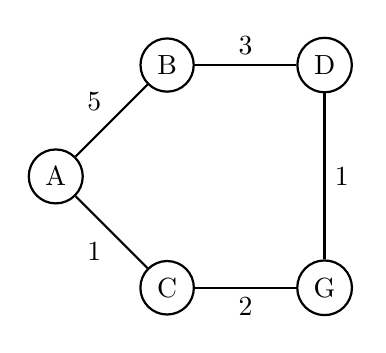
\begin{tikzpicture}[node distance={2cm}, thick, main/.style = {draw, circle}] 
			\node[main] (A) {A};
			\node[main] (B) [above right of=A] {B};
			\node[main] (C) [below right of=A] {C};
			\node[main] (D) [right of=B] {D};
			\node[main] (G) [right of=C] {G};
			
			\path (A) edge node[above left] {5} (B);
			\path (A) edge node[below left] {1} (C);
			\path (B) edge node[above] {3} (D);
			\path (C) edge node[below] {2} (G);
			\path (D) edge node[right] {1} (G);
		\end{tikzpicture}
		\caption{Example graph for UCS demonstration (Numbers represent edge costs)}
		\label{fig:ucs_graph}
	\end{figure}
	
	\subsubsection{Algorithm Steps}
	\begin{enumerate}[label=\textbf{Step \arabic*}:]
		\item Initialize priority queue with start node (cost = 0)
		\item While queue is not empty:
		\begin{itemize}
			\item Dequeue node with \textbf{lowest cumulative cost}
			\item If goal node found, return path
			\item Expand to neighboring nodes
			\item Enqueue neighbors with updated path cost
		\end{itemize}
		\item If queue empties, return failure
	\end{enumerate}
	
	\subsection{Complexity Analysis}
	\begin{itemize}
		\item \textbf{Time Complexity}: $O((E + V)\log V)$ \\ 
		Where $E$ = edges, $V$ = vertices. Uses priority queue (typically binary heap)
		
		\item \textbf{Space Complexity}: $O(V)$ \\
		Stores all nodes in worst case
	\end{itemize}
	
	\subsection{Optimality and Completeness}
	\begin{itemize}
		\item \textbf{Optimal}: Always finds least-cost path when:
		\begin{itemize}
			\item All edge costs are non-negative
			\item Path cost increases with depth
		\end{itemize}
		
		\item \textbf{Complete}: Guaranteed to find solution if one exists
	\end{itemize}
	
	\subsection{Comparison with Other Algorithms}
	\begin{itemize}
		\item \textbf{vs BFS}: UCS generalizes BFS (BFS uses edge count as cost)
		\item \textbf{vs Dijkstra's}: Essentially identical - both find shortest paths
		\item \textbf{vs A*}: A* uses heuristics to guide search, UCS is heuristic-free
	\end{itemize}
	
	\section{Implementation}
	
	This code implements the Uniform Cost Search (UCS) algorithm to find the shortest path between two nodes in a weighted graph. UCS is a graph traversal algorithm that finds the path with the lowest cumulative cost from a starting node to a goal node.
	
	\subsection{Code Structure}
	
	The core of the implementation is the \texttt{uniform\_cost\_search(graph, start, goal)} function:
	
	\begin{itemize}
		\item \textbf{Input:} A graph \texttt{graph}, a starting node \texttt{start}, and a goal node \texttt{goal}.
		\item \textbf{Data Structures:}
		\begin{itemize}
			\item \texttt{priority\_queue}: A min-heap (implemented using \texttt{heapq}) storing tuples of \texttt{(cumulative\_cost, current\_node, path)}.
			\item \texttt{visited}: A dictionary storing the minimum cost to reach each visited node.
		\end{itemize}
		\item \textbf{Algorithm:}
		\begin{enumerate}
			\item Initialize the \texttt{priority\_queue} with the starting node and a cost of 0.
			\item While the \texttt{priority\_queue} is not empty:
			\begin{enumerate}
				\item Pop the node with the lowest cumulative cost.
				\item If the current node is the goal, construct the path and return it along with the total cost. Color the path edges green in the graph.
				\item If the current node has been visited with a lower cost, skip it.
				\item For each neighbor of the current node:
				\begin{enumerate}
					\item Calculate the cost to reach the neighbor.
					\item If the neighbor is unvisited or the new cost is lower than the previously recorded cost, add it to the \texttt{priority\_queue}.
				\end{enumerate}
			\end{enumerate}
			\item If the goal is not reachable, return \texttt{None} and infinity.
		\end{enumerate}
		\item \textbf{Output:} A tuple containing the path (list of nodes), the total cost, and the graph with colored path edges.
	\end{itemize}
	
	\subsection{Key Concepts}
	
	\begin{itemize}
		\item \textbf{Priority Queue:} Ensures that nodes with the lowest cost are explored first.
		\item \textbf{Visited Set:} Prevents revisiting nodes along suboptimal paths, improving efficiency.
		\item \textbf{Graph Representation:} Uses \texttt{networkx} to represent the graph, allowing for weighted edges.
	\end{itemize}
	
	This implementation provides an efficient way to find the shortest path in a weighted graph using the Uniform Cost Search algorithm.
	
	\subsection{Output Interpretation}
	
	\begin{table}[htbp]
		\centering
		\caption{Search Algorithm Comparison}
		\begin{tabular}{lcccccc}
			\toprule
			\multirow{2}{*}{Nodes} & \multicolumn{2}{c}{UCS} & \multicolumn{2}{c}{BFS} & \multicolumn{2}{c}{DFS} \\
			\cmidrule(lr){2-3} \cmidrule(lr){4-5} \cmidrule(lr){6-7}
			& Time (s) & Path Length & Time (s) & Path Length & Time (s) & Path Length \\
			\midrule
			50   & 0.001392 & 4           & 0.001102 & 4           & 0.000878 & 4           \\
			100  & 0.001709 & 6           & 0.001733 & 4           & 0.001799 & 23          \\
			200  & 0.004672 & 6           & 0.003726 & 6           & 0.003607 & 52          \\
			400  & 0.005482 & 0           & 0.005958 & 0           & 0.005479 & 0           \\
			800  & 0.014376 & 8           & 0.015159 & 7           & 0.018944 & 424         \\
			1000 & 0.023005 & 8           & 0.018543 & 6           & 0.021258 & 412         \\
			1500 & 0.041061 & 12          & 0.028889 & 8           & 0.062434 & 862         \\
			\bottomrule
		\end{tabular}
	\end{table}
	
	\section{Applications}
	\begin{itemize}
		\item Network routing protocols
		\item GPS navigation systems
		\item Robotics path planning
		\item Puzzle solving (e.g., sliding tile puzzles)
	\end{itemize}
	
	\section{Conclusion}
	Uniform Cost Search provides an optimal solution for pathfinding in weighted graphs with non-negative edge costs. While not as fast as heuristic-based methods like A* for many problems, it remains fundamental in AI due to its guaranteed optimality and simplicity.
	
\end{document}